\documentclass[twocolumn,11pt]{jarticle}

\usepackage[dvipdfmx]{graphicx}
\graphicspath{ {math-images4/} }
\usepackage[dvipdfmx]{color}
\usepackage{geometry}
\usepackage{amsmath}
\usepackage{latexsym}
%\usepackage{ascmac}
\usepackage{fancyhdr}
\usepackage{overpic}
\usepackage[dvipdfmx,%
 bookmarks=true,%
 bookmarksnumbered=true,%
 colorlinks=true,%
 linkcolor=blue,%
 setpagesize=false,%
 pdftitle={数学の基礎訓練IV},%
 pdfauthor={西井淳},%
 pdfsubject={数学の基礎訓練IV},%
 pdfkeywords={応用数学}]{hyperref}
\usepackage{pxjahyper}%hyperrefの不具合対応
\usepackage{makeidx} %索引
\usepackage{mymath}
\makeindex

\geometry{body={178mm,242mm},columnsep=9mm}


\begin{document}

\pagestyle{empty}
\twocolumn[
\noindent
\rule{\linewidth}{0.5pt}
\begin{center}
{\Huge\gtfamily 数学の基礎訓練IV\\
\LARGE 〜応用編〜}
\end{center}
\begin{flushright}
\today 版\quad 西井 淳
\\
\rule{\linewidth}{0.5pt}
\end{flushright}
{\small\tableofcontents}
]

\newpage

\rule{0pt}{10cm}
\newpage

\setcounter{page}{1}
\pagestyle{fancy}

\section{フーリエ級数・フーリエ変換}

\subsection{関数の内積}

区間$[a,b]$で定義される積分可能な二つの関数$f(x),g(x)$の内
積$<f(x),g(x)>$を以下のように定義することにする。
\begin{align}
  <f(x),g(x)>=\int_{a}^{b}f(x)g^*(x)dx \notag
\end{align}
ここで,$g^*(x)$は$g(x)$の共役複素数である。
内積$<f(x),g(x)>$が0になるときには,$f(x)$と$g(x)$は直交すると言う。

\question
関数$s_n(x)=\sin nx$, $c_m(x)=\cos mx$, ($n$, $m$は整数)に関
し,区間$[-\pi,\pi]$における内積が以下のようになることを証明しなさい。
以下で$\delta_{nm}$は\bfindex{クロネッカーのデルタ}
(\nmindex{Kronecker's delta})である
\footnote{
クロネッカーのデルタ$\delta_{nm}$とは以下で定義される。
$\delta_{nm}=
\begin{cases}
  1&(n=m)\\
  0 &(n\ne m)
\end{cases}
$
}。
\begin{enumerate}
\item $<s_n(x), s_m(x)>=\pi\delta_{nm}$
\item $<c_n(x), c_m(x)>=2\pi\delta_{nm} $
\item $<s_n(x), c_m(x)>=0$
\end{enumerate}
この問の結果より,$\sin nx$, $\cos mx$は
区間$[-\pi,\pi]$において
\bfindex[ちょっこうかんすうけい]{直交関数系}
(自分自身との内積以外はすべて$0$となる関数系)であることがわかる。

\subsection{フーリエ級数展開}

ある楽器の音を人工的に合成する方法を考えてみよう。
サンプリングした楽器の音を$y=f(t)$とし,これはある周期$T$をもつ信号と
仮定する。
このとき楽器の音は基調となる周波数($f=1/T$)とその倍音成分の重ね合わせ,
すなわち次式で表現できると考えられる。
\begin{align}
  \label{eq:FourierT}
  f(t)=\sum_{n=0}^{\infty} 
  (a_n\cos 2\pi n\frac{t}{T} + b_n \sin 2\pi n\frac{t}{T}).
\end{align}
このように正弦波の組合せで任意の信号を表現できれば,その合成は大変容易
になる。
どのようにしたら各係数を決定できるだろうか。

\nquestion
式(\ref{eq:FourierT})において簡単のため関数$y=f(t)$が周期$2\pi$である
とした場合、すなわち、
\begin{align}
  f(t)=\sum_{n=0}^{\infty} (a_n\cos nt + b_n \sin nt)
  \label{eq:Fourier2pi}
\end{align}
の各係数$a_n,b_n$を求める式を導出しなさい。

\comment
このように,周期$2\pi$の関数$f(x)$を直交関数系$\sin nx$, $\cos mx$で展
開することを\bfindex[ふーりえきゅうすうてんかい]{フーリエ級数展開}という。

フーリエ級数展開を行うと,信号のもつ各周波数成分の大きさを計算できる。
すなわち,$n$次周波数成分の大きさは$a_n^2+b_n^2$で与えられる。
すなわち,フーリエ級数展開は,信号の周波数分析を行うための基本的手法で
ある。


\nquestion
\begin{enumerate}
\item $a_0$は関数$f(x)$のどのような性質を表すか?
\item 奇関数をフーリエ級数展開すると$a_n=0$となることを示しなさい。
\item 偶関数をフーリエ級数展開すると$b_n=0$となることを示しなさい。
  \end{enumerate}

\exercise
次式について以下の問に答えなさい。
  \begin{align}
    \label{eq:qfourier}
    f(x)=
    \begin{cases}
      1 & (-\pi\le x<0)\\
      0 & (0\le x<\pi)
    \end{cases}
  \end{align}
\begin{enumerate}
\item フーリエ級数展開せよ。
\item 上で求めたフーリエ級数において,周波数成分が高くなるにつれ,各成
  分の大きさがどうかわるかを図示して示しなさい。
\item 上で求めたフーリエ級数において,(i) 1次までの項のみ,(ii) 2次ま
  での項のみ,
  (iii) 3次までの項のみを考えた場合について,元の式
  (\ref{eq:qfourier})をどの程度表現しているか,グラフを書いて確認せよ。
\end{enumerate}

\subsection{複素フーリエ級数展開}

\nquestion
オイラーの公式より次式が成立する。
\begin{align}
  \cos a&=\frac{e^{ia}+e^{-{ia}}}{2}\\
  \sin a&=\frac{e^{ia}-e^{-{ia}}}{2i}
\end{align}
上式を用いると式(\ref{eq:FourierT})を次式のように書けることを示しなさ
い。
\begin{align}
  f(t)=\sum_{n=-\infty}^{\infty} c_ne^{in\omega t},\quad(\omega=\frac{2\pi}{T})
  \label{eq:FourierE}
\end{align}
また,$c_n$と$a_n$, $b_n$の関係式を書きなさい。

\comment
上式のように複素数表現によるフーリェ級数展開を
\bfindex[ふくそふーりえきゅうすうてんかい]{複素フーリェ級数展開}という。

\nquestion
関数$e^{in\omega t}$, $(\omega=\frac{2\pi}{T}$, 
$n=0,\pm 1, \pm2, \cdots)$が
区間$[-\frac{T}{2},\frac{T}{2}]$において直交関数系であることを示しなさい。

\nquestion
式(\ref{eq:FourierE})の係数$c_n$を次式で求めることができることを示しな
さい。
\begin{align}
  \label{eq:fourierCn}
  c_n=\frac{1}{T}\int_{-\frac{T}{2}}^{\frac{T}{2}}f(t)e^{-in\omega t}dt
\end{align}
ここで,$|c_n|=\sqrt{c_nc_{-n}}(=\sqrt{a_n^2+b_n^2})$は周期$T$の関数に
含まれる$n$次周波数成分(周期 が$\frac{T}{n}$の振動成分)の大きさを表す。

\subsection{フーリエ変換}
周期$T$の信号に含まれる高次周波数成分の周期$T_n$は離散的な値
($T_n=\frac{n}{T}$, $n=0,1,2,\cdots$)をとり,
その$n$次周波数成分の大きさは式(\ref{eq:fourierCn})で計算可能である。
一方,一定の周期をもたない信号$f(t)$を周期無限長の信号と考えると,
そこに含まれる周波数成分の周期は連続な分布になる。
そして、ある周期$T$(角速度$\omega=2\pi/T$)の周波数成分の大きさ$F(\omega)$
は式(\ref{eq:fourierCn})の右辺とほぼ同様に次式で与えられる。
\begin{align}
  F(\omega)=\int_{-\infty}^{\infty}f(t)e^{-i\omega t}dt
  \label{eq:Fourier}
\end{align}
これを関数$f(t)$の\bfindex[ふーりえへんかん]{フーリエ変換}とよぶ。
また,フーリエ変換の逆変換である
\bfindex[ぎゃくふーりえへんかん]{逆フーリエ変換}は次式で与えられる。
\begin{align}
  f(t)=\frac{1}{2\pi}\int_{-\infty}^{\infty}F(\omega)e^{i\omega t}d\omega
  \label{eq:inv-Fourier}
\end{align}

ただし,フーリエ変換の係数の付け方にはいろいろなお流儀があり、例えば以
下のように定義される場合もある。
\begin{align}
  F(\omega)=\frac{1}{\sqrt{2\pi}}\int_{-\infty}^{\infty}f(t)e^{-i\omega t}dt
  \notag
\end{align}
この場合には逆フーリエ変換は次のようになる。
\begin{align}
  f(t)=\frac{1}{\sqrt{2\pi}}\int_{-\infty}^{\infty}F(\omega)e^{i\omega t}d\omega
  \notag
\end{align}

\nquestion
以下を満たす関数$\delta(x)$を
\bfindex[でぃらくのでるたかんすう]{ディラクのデルタ関数}とよぶ。
\begin{align}
  \begin{cases}
  &\delta(x)=0\quad  (x\ne 0)\notag\\
  &\displaystyle\int_{-\infty}^{\infty}\delta(x)dx=1
  \end{cases}
\end{align}
デルタ関数は以下のような関係式をみたす。
\begin{align}
  \int_{-\infty}^{\infty}\delta(x)f(x)dx=f(0)\notag
\end{align}
\begin{enumerate}
\item デルタ関数$\delta(t)$のフーリエ変換を求めなさい。
  また,その結果の意味を説明しなさい。
\item デルタ関数$\delta(\omega)$の逆フーリエ変換を求めなさい。
  また,その結果の意味を説明しなさい。
\item 以上の結果をもとに$f(t)=e^{iat}$のフーリエ変換を求めなさい。
\item 式(\ref{eq:Fourier})の逆変換が式(\ref{eq:inv-Fourier})で与えられ
  ることを証明しなさい。(式(\ref{eq:Fourier})を逆フーリエ変換すれば
  $f(t)$が得られる事を証明する。)
\end{enumerate}

\nquestion
以下のフーリエ変換を求めなさい。
\begin{enumerate}
\item $f(t)=\sin t$
\item $f(t)=\cos t$
\item $f(t-T)$, \quad($f(t)$のフーリエ変換を$F(\omega)$とおく)
\end{enumerate}

% \newpage
% \rule{0pt}{20cm}
\newpage

\section{微積分の応用}

\subsection{微分の数値計算}
\nquestion
関数$f(x)$を$x=x_n$のまわりでテイラー展開し,
  $f(x_{n+1})$および$f(x_{n-1})$を$f(x_n)$, $f'(x_n)$, $f''(x_n)$を用いて表せ。
  ここで,$x_{n\pm 1}=x_n\pm h$ ($h\ll 1$)である。

\nquestion
先の結果より以下を導け。
  \begin{enumerate}
  \item \bfindex[ぜんしんさぶん]{前進差分}の式
    \begin{align}
      f'(x_n)=\frac{f(x_{n+1})-f(x_n)}{h}+O(h)\notag
    \end{align}
  \item \bfindex[こうたいさぶん]{後退差分}の式
    \begin{align}
      f'(x_n)=\frac{f(x_{n})-f(x_{n-1})}{h}+O(h)\notag
    \end{align}
  \item \bfindex[ちゅうしんさぶん]{中心差分}の式
    \begin{align}
      f'(x_n)=\frac{f(x_{n+1})-f(x_{n-1})}{2h}+O(h^2)\notag
    \end{align}
  \item 2階微分
    \begin{align}
      f''(x_n)=\frac{f(x_{n+1})-2f(x_n)+f(x_{n-1})}{h^2}+O(h^2)\notag
    \end{align}
  \end{enumerate}

\nquestion
時系列データ
  $x_0=x(0)$, $x_1=x(h)$, $\ldots$, $x_n=x(nh)$, $\ldots$が得られたと
  き,時刻$t=nh$における微分を最も精度よく求めるにはどうしたらよいか。
  前問の結果より理由と共に答えよ。

\nquestion
$f(x)=x^2$の$x=0$および$x=0.1$における微分値を求めたい。
  \begin{enumerate}
  \item $f(x)$を微分することにより,$f'(0)$, $f'(0.1)$を求めなさい。
  \item $f(-0.1)$, $f(0)$, $f(0.1)$, $f(0.2)$の値を用い,
    前進差分,後退差分,中心差分それぞれにより$f'(0)$, $f'(0.1)$を近似
    的に求めなさい。またその結果を考察しなさい。
  \end{enumerate}

\section{微分方程式}

\subsection{力学系入門}

\begin{enumerate}
\item $\dot{x}>0$の場合,$x$は時間とともに増えるだろうか,それとも減る
  だろうか。$|\dot{x}|$の大きさにより,$x$の時間変化の割合はどう違うだ
  ろうか。理由とともに述べなさい。
%% 微分方程式$\dot{x}=-x$の解の軌跡を,横軸を時刻$t$, 縦軸を$x$として
%%   図示せよ(\textbf{解を求めずに}グラフを考える)。
%%   また解を求め,先に図示した軌跡と一致することを確認せよ。
\item 微分方程式
  \begin{align}
    \label{eq:logistic}
    \dot{x}=(1-x)x
  \end{align}
  について以下の問に答えよ。
  \begin{enumerate}
  \item $\dot{x}=0$ を満たす$x$を求めよ。このような点を
    \bfindex[へいこうてん]{平衡点}(\nmindex{equilibrium point})と呼ぶ。
  \item 横軸に$x$, 縦軸に$\dot{x}$をとったときの式(\ref{eq:logistic})
    のグラフをかけ。
\item 
  平衡点のうち,わずかな摂動で
  離れる点を\bfindex[ふあんていてん]{不安定点}
  (\nmindex{unstable point}), 
  摂動があってももとに戻る点を\bfindex[あんていてん]{安定点}
  (\nmindex{stable point})と呼ぶ。
  各平衡点の安定性を前問のグラフから判断せよ。
\item 以上の結果を参考にして,解の軌跡を図示せよ。
  (横軸に時間,縦軸に$x$をとったグラフをつくる) 
\item $f(x)=(1-x)x$とおいたとき,平衡点における$f'(x)$を求めよ。
  その符合と平衡点の性質の関連を考えよ
  \item 以上の結果を参考にして,解の軌跡を図示せよ。
    (横軸に時間,縦軸に$x$をとったグラフをつくる) 
  \item $f(x)=(1-x)x$とおいたとき,平衡点における$f'(x)$を求めよ。
    その符合と平衡点の性質の関連を考えよ
  \end{enumerate}
\item 以下の各微分方程式における平衡点とその安定性,解の挙動を議論せよ。
解を陽に求めることなく議論すること。
  \begin{enumerate}
  \item $\dot{x}=x$
  \item $\dot{x}=1-x$
%   \item $\dot{x}=\sin x$
  \item $y'=y^2-3y+2$
  \end{enumerate}

\end{enumerate}


%\subsection{微分方程式の基本}

\subsection{変数分離型微分方程式}
以下の微分方程式の解を求めよ。また,求めた解を微分方程式に代入す
ることにより検算せよ
\answer{
(\ref{item:dy+ay}) $y=Ce^{-ax}$~
(\ref{item:dy-xy}) $y=Ce^{\frac{1}{2}x^2}$~
(\ref{item:dv+av-b}) $v=\frac{b}{a}+Ce^{-at}$~
(\ref{item:dy-x(1-y)}) $y=1+C e^{-\frac{1}{2}x^2}$
(\ref{item:dy-4x3y}) $y=Ce^{x^4}$
(\ref{item:dy+ytanx}) $y=C\cos x$
(\ref{item:dx-sinx}) $\tan\frac{x}{2}=Ce^t$
(\ref{item:dx-(a-bx)x}) $x=\frac{a}{b}\frac{1}{1-Ce^{-at}}$
(\ref{item:yydy+xy3-x}) $y=\sqrt[3]{1+Ce^{-\frac{3}{2}x^2}}$
(\ref{item:dysqrt(x-1)-sqrt(y-1)}) $\sqrt{y-1}=\sqrt{x-1}+C$, $y=1$
}。
\begin{enumerate}
\item \label{item:dy+ay}$y'=-ay$, ($a:$ 定数)
\item \label{item:dy-xy}$y'=xy$
\item \label{item:dv+av-b}$\dot{v}=-av+b$, \quad($a,b:$ 定数)
\item \label{item:dy-x(1-y)}$y'=x(1-y)$
\item \label{item:dy-4x3y}$y'-4x^3y=0$
\item \label{item:dy+ytanx}$y'+y\tan x=0$
\item \label{item:dx-sinx}$\dot{x}=\sin x$
\item \label{item:dx-(a-bx)x}$\dot{x}=(a-bx)x$, \quad($a,b:$ 定数)
\item \label{item:yydy+xy3-x}$y^2y'+xy^3=x$
\item \label{item:dysqrt(x-1)-sqrt(y-1)}$y'\sqrt{x-1}-\sqrt{y-1}=0$
\end{enumerate}

\subsection{線形微分方程式}

\subsubsection{斉次微分方程式}
以下の二階斉次線形微分方程式の解を求めたい。
\begin{align}
\label{eq:2diffeq}
\ddot{x}+a\dot{x}+bx=0
\end{align}
\begin{enumerate}
\item 微分方程式の解を$x=Ce^{\lambda t}$と仮定し,実際にこれが式
  (\ref{eq:2diffeq})の解となるには$\lambda$がどのような条件を満たせ
  ばよいかを議論しなさい。

  \comment
  $x=Ce^{\lambda t}$が式(\ref{eq:2diffeq})の解となるために$\lambda$が
  満たすべき方程式を\bfindex[とくせいほうていしき]{特性方程式}という。
\item 特性方程式の解を$\lambda_1$, $\lambda_2$とすると,
  微分方程式の解は次のようになることを示しなさい。
  \begin{enumerate}
  \item $\lambda_1\ne\lambda_2$の時
    \begin{align}
      x=C_1e^{\lambda_1t}+C_2e^{\lambda_2t}\notag
    \end{align}
    ただし,$\lambda=\alpha\pm i\omega$, ($\omega\ne 0$)の場合には
    以下のように書けることを示しなさい。
    \begin{align}
      x=e^{\alpha t}(C_1\cos{\omega t}+C_2\sin{\omega t})\notag
    \end{align}
  \item $\lambda_1=\lambda_2$の時
    \begin{align}
      x=(C_1+C_2t)e^{\lambda_1t}\notag
    \end{align}
  \end{enumerate}
\item 解の振舞を$a$, $b$の値によって分類し,図示して説明しなさい。
\end{enumerate}

\exercise
以下の微分方程式の解をそれぞれ求め,解軌道を図示しなさい。
また,求めた解を微分方程式に代入することにより検算をしなさい。
\begin{enumerate}
\item $y''+6y'+5y=0$
\item $y''-4y=0$
\item $y''+4y=0$
\item $\ddot{x}+4\dot{x}+5x=0$
\item $\ddot{x}+2\dot{x}+x=0$
\end{enumerate}

\subsubsection{非斉次微分方程式}
以下の二階非斉次微分方程式の解を求めよう。
\begin{align}
\label{eq:inhomogeneous}
\ddot{x}-3\dot{x}+2x=e^{-t}
\end{align}

\begin{enumerate}
\item 式(\ref{eq:inhomogeneous})を斉次微分方程式に修正した次式の解を求
  めなさい。
\begin{align}
\ddot{x}-3\dot{x}+2x=0
\end{align}
\comment ここで求めた解を$x=x_p$とおく。
  これを式(\ref{eq:inhomogeneous})の左辺に代入して整理すれば零にな
  る。この解を式(\ref{eq:inhomogeneous})の\textbf{一般解}と呼ぶ。
  式(\ref{eq:inhomogeneous})の解はさらに特解$x=x_s$を加えた
  $x=x_p+x_s$という形になる。ここで特解$x=x_s$は
  式(\ref{eq:inhomogeneous})を満たす解である。

  特解を求めるには左辺に代入したときに右辺の$e^{-t}$になる関数は何か
  あたりをつけることから始める。
  この場合は$x_s=ae^{-t}$という形にすれば良いかもと考え、これを
  式(\ref{eq:inhomogeneous})に代入し、$a$の値を求める。
  その結果どのような$a$を与えても式(\ref{eq:inhomogeneous})を満足出来
  ない場合には、特解の形を考え直す。
\item 式(\ref{eq:inhomogeneous})の特解を求めなさい。本問と前問の結果よ
  り式(\ref{eq:inhomogeneous})の解を述べなさい。
\end{enumerate}

\exercise
\begin{enumerate}
\item 以下の微分方程式の解をそれぞれ求め,解軌道を図示しなさい。
  また,求めた解を微分方程式に代入することにより検算をしなさい。
  \begin{enumerate}
  \item $\ddot{x}+2\dot{x}+x=1$
  \item $y'-5y=1$
  \item $y''-5y'+6y=1$
  \item $y''+4y'+3y=x$
  \item $\dot{x}+4x=\cos 2t$
  \item $\ddot{x}+5\dot{x}+4x=\cos 2t$
  \item $y''-5y'+4y=x+\sin x$
  \end{enumerate}
  %% \item 微分方程式 $\ddot{x}+a\dot{x}+bx=\sin \omega t$ の解を求めよ。また,
  %%   その振舞いを論じよ。
\item 以下の微分方程式について各問に答えよ。
  \begin{align}
    \begin{cases}
      \dot{x}&=y\\
      \dot{y}&=-x
    \end{cases}\notag
  \end{align}
  \begin{enumerate}
  \item 上式にもとづいて$x$と$y$が変化するとき,$x^2+y^2$の値は時間と
    ともにどのように変わるかを解析的に検討しなさい
    \footnote{ヒント)$V=x^2+y^2$の時間微分を求める}。
    また,その結果の幾何学的意味を説明しなさい。
  \item 微分方程式を解き,$x$, $y$を時間の関数として求めよ。
    その解が前問で答えた特徴を満たしていることを確認せよ。
  \end{enumerate}
\end{enumerate}
% \item 次の微分方程式について以下の問に答えよ。
% \begin{align}
%   \label{eq:lotka-volterra}
%   \begin{cases}
%     \dot{x}=x(1-ay)\\
%     \dot{y}=-y(1-bx) \notag
%   \end{cases}
% \end{align}


\subsection{微分方程式と定性的表現}
ある島に住むうさぎは個体数に比例する増加率を示す。
その増加率を決める比例定数はえさの量がある値より大きいかどうかで決まる。
以下の各状況を微分方程式を用いて議論せよ。
\begin{enumerate}
\item 一匹あたりのえさの量が常に一定であれば,うさぎの数はどのように推移す
  ると考えられるか?
\item 一匹あたりのえさの量が,個体数が多いときには少なくなるならば、うさ
  ぎの数はどのように推移すると考えられるか?
\end{enumerate}



\section{多変数関数の微分}

\subsection{偏微分}
\begin{enumerate}
\item 2変数関数$z=f(x,y)$の$x$\bfindex[へんどうかんすう]{偏導関数}
(\nmindex{partial derivative})
(一般に$\frac{\partial f}{\partial x}$, $f_x$と書く)の定義を書きなさい
\item $f(x,y)=x^2+2y^2$に関して以下の問に答えなさい。
  \begin{enumerate}
  \item 関数$f(x,y)$を平面$x=2$で切った断面の方程式とグラフを書きなさ
    い。また,この断面を表すグラフの$y=2$における傾きを求めなさい。
  \item 偏微分$f_x$, $f_y$を求めなさい。そのいずれかを用いることで前問
    で求めた傾きを求めることができることを説明しなさい。
  \end{enumerate}
\end{enumerate}% 

\subsection{勾配}

一般に関数$f$の\bfindex[こうばい]{勾配}(\nmindex{gradient})を$\grad f$と表す。
3変数関数$f(x,y,z)$の勾配も前問と同様に考えると,次式のように表される。
\begin{align}
\grad f=\left(\frac{\partial f}{\partial x},\frac{\partial f}{\partial
  y},\frac{\partial f}{\partial z}\right)\notag
\end{align}
ここでベクトル演算子
$\nabla=\left(\frac{\partial}{\partial x},\frac{\partial}{\partial
  y},\frac{\partial}{\partial z}\right)$
を用いると,
\begin{align}
\nabla f=\grad f
=\left(\frac{\partial f}{\partial x},\frac{\partial f}{\partial
  y},\frac{\partial f}{\partial z}\right)\notag
\end{align}
と書ける。演算子$\nabla$は"\bfindex{ナブラ}"と呼ばれる記号だが,上記のように
勾配を表すときには"gradient"と読む。

関数$\displaystyle\phi(\boldsymbol{r})=\frac{1}{r}$, $\boldsymbol{r}=(x,y,z)$, 
$(r=|\boldsymbol{r}|, r\ne0)$に関して以下の問いに答えよ。

\begin{enumerate}
\item $\boldsymbol{f}=-\nabla\phi$を求めよ。
\item $\boldsymbol{f}$はどのような大きさと方向を持つベクトルか,図示し
  て説明せよ。
  説明においては,関数$\phi$の等高線の概形との関係に注意すること。 
\end{enumerate}

%\subsection{発散}
%
%演算子$\nabla$は,ベクトル関数$(f_x,f_y,f_z)$
%
%\begin{enumerate}
%\item $\boldsymbol{f}$の発散$\nabla\cdot\boldsymbol{f}=-\nabla\cdot\nabla\phi$を求めよ。
%\end{enumerate}% 

\subsection{全微分}

\begin{enumerate}
\item 関数$z=f(x,y)$が,点$(a,b,f(a,b))$において$xy$平面と垂直
  でない\bfindex[せつへいめん]{接平面}をもつとき,
  $f(x,y)$は$(a,b)$で\bfindex[ぜんびぶんかのう]{全微分可能}であるという。
  この接平面の方程式を書きなさい。

  (ヒント:接点において,$z=f(x,y)$とその接平面の各偏導関数の値は等し
  くなる)
\item 関数$z=f(x,y)$が全微分可能であるとする。
  $(x,y)\rightarrow (x+dx,y+dy$)と変化したとき,
  関数$z=f(x,y)$の$(x,y,f(x,y))$における接平面上の$z$座標の変化量$dz$
  \begin{align}
    dz=f(x+dx,y+dy)-f(x,y)\notag
  \end{align}
  が,$dx$, $dy$が十分小さいときには次式で近似できることを説明せよ。
  \begin{align}
    dz&=f_x(x,y)dx+f_y(x,y)dy\notag\\
    &=(\nabla {f}(\vect{x}),\Delta \vect{x})\notag
  \end{align}
  \comment
  ベクトル$\nabla f(\vect{x})=(f_x,f_y)$は,関数$f$の$(x,y)$における
  \bfindex[さいきゅうこうばい]{最急勾配}(単に勾配ということが多い)の方
  向を表すことになる。
  このように与えられる$dz$を$f(x,y)$の\bfindex[ぜんびぶん]{全微分}
  (\nmindex{total derivative})という。
  $dx\to 0,dy\to 0$のとき,
  $x,y$の微小増加分に対する関数$f(x,y)$の変化量$dz$
  は全微分で与えられる。
\item 関数$z=f(x,y)$について、ある点$(x,y)$における\textbf{最急勾配}の
  方向と高さ一定の方向は直交することを示しなさい。
\item 次式の全微分を求めよ
  \begin{enumerate}
  \item $z=e^{-x^2y}$
  \item $\displaystyle z=\frac{1}{x^2+y^2}$
  \item ばね定数$k$のばねの先に質量$m$のおもりがついているとき,そのば
    ねの固有周期$T$は$T=2\pi\sqrt{\frac{k}{m}}$で与えられる。
    ばね定数$k$や質量$m$の微少変化$\frac{dk}{k}$,$\frac{dm}{m}$に対す
    る固有周期の変化$\frac{dT}{T}$を全微分を用いて説明しなさい。
  \end{enumerate}
\end{enumerate}
\comment
より一般になめらかな関数$f(x,y,z)=0$上で変位
$(x,y,z)\rightarrow(x+dx,y+dy,z+dz)$したとき,% 

\subsection{ラグランジュの未定乗数法}

拘束条件
\begin{align}
\label{eq:lagrange-g}
&g(x,y)=0
\end{align}
のもとで
\begin{align}
\label{eq:lagrange-f}
z=f(x,y)
\end{align}
の極値を与える点$(a,b)$を求めたい。

式(\ref{eq:lagrange-g})を全微分すると
\begin{align}
  \label{eq:lagrange-g2}
  g_{x}dx+g_{y}dy=0
\end{align}
ここで,上式は式(\ref{eq:lagrange-g})を満たすための変数$x,y$間の拘束条
件を表している。

次に式(\ref{eq:lagrange-f})を全微分すると
\begin{align}
  dz=f_{x}dx+f_{y}dy\notag
\end{align}
全微分$dz$は極値$(a,b)$において0になるので,
\begin{align}
  \label{eq:lagrange-f2}
  f_{x}dx+f_{y}dy=0.
\end{align}
式(\ref{eq:lagrange-g2})(\ref{eq:lagrange-f2})を$dx,dy$を変数とする連
立方程式と捉えると次式のように書くことができる。
\begin{align}
  \begin{pmatrix}
    g_x & g_y\\
    f_x & f_y
  \end{pmatrix}
  \begin{pmatrix}
    d_x \\ d_y
  \end{pmatrix}
  =
  \begin{pmatrix}
    0 \\ 0
  \end{pmatrix}\notag
\end{align}
極値$(a,b)$において$(dx,dy)=(0,0)$以外の解をもつ条件は,上式の
係数行列が非正則であることである。
このとき,ある定数$\lambda$が存在して,
\begin{align}
\label{eq:lagrange}
  \begin{cases}
  f_x-\lambda g_x=0\\
  f_y-\lambda g_y=0
  \end{cases}
\end{align}
が成立する。
この2式と式(\ref{eq:lagrange-g})の3式を連立方程式として解くこ
とにより,極値における3変数$(x,y,\lambda)$の値を求めることができる。
これが\textbf{ラグランジュの未定乗数法}
\index{ラグランジュ!のみていじょうすうほう@---の未定乗数法}であり,
$\lambda$を\textbf{ラグランジュ乗数}
\index{ラグランジュ!じょうすう@---乗数}であり,
とよぶ。
$f$,$g$が3変数以上の多変数関数の場合にもラグランジュの未定
乗数法を適用できることを同様に証明できる。

ちなみに,式(\ref{eq:lagrange})は次のように書くこともできる。
\begin{align}
\nabla f -\lambda \nabla g=0\notag.
\end{align}
この式は\textbf{ある点における関数$f(x,y)$と$g(x,y)$の接線の法線ベクトルが同じ
向きである}こと、すなわち両者の接線(3変数以上の場合は接平面)が一致することを示す。


\nquestion
\begin{enumerate}
\item $x+y+z=1$のもとで,$f(x,y,z)=x^2+y^2+z^2$を最小にする$(x,y,z)$を
  ラグランジュの未定乗数法を用いて求めよ。
\item 前問の結果の幾何学的意味を考えよ。
\end{enumerate}
\nquestion
\begin{enumerate}
\item $x+y+z=1$上の点のうち点$P(1,2,3)$までの距離を最小にする点$Q$とそ
  の距離をラグランジュの未定乗数法を用いて求めよ。
\item 前問の結果の幾何学的意味を考えよ。
  特に線分$PQ$と平面$x+y+z=1$はどのような関係になっているかを述べよ。
\end{enumerate}
% 

\subsection{2変数関数のテイラー展開}
$C^{\infty}$級2変数関数$z=f(x,y)$を,点P$(a,b)$において
\bfindex[ていらーてんかい]{テイラー展開}(\nmindex{Taylor expansion})を
行うことにより無限級数に展開すると次式のようになる。 
\begin{align}
  f(x+a&,y+b)
  =f(a,b)\notag\\
  &+\left(x\frac{\partial}{\partial x}+y\frac{\partial}{\partial y}\right)f(a,b) \notag\\
  &+\frac{1}{2!}\left(x\frac{\partial}{\partial x}+y\frac{\partial}{\partial y}\right)^2f(a,b) \notag\\
  &+\cdots \notag\\
  &+\frac{1}{n!}\left(x\frac{\partial}{\partial x}+y\frac{\partial}{\partial y}\right)^nf(a,b) \notag\\
  &+\cdots \notag\\
  =&\sum_{n=0}^{\infty}
   \frac{1}{n!}\left(x\frac{\partial}{\partial x}+y\frac{\partial}{\partial y}\right)^{n}f(a,b)
 \notag
\end{align}
\question
1変数関数のテイラー展開と同様の考え方により上式を導けることを$n=2$の
項まで確認しなさい。

%% \section{ついでに物理の基礎}
%% \subsection{単位}
%% \nquestion

%% MKSA単位とCGSA単位とはなにか,簡単に説明せよ。
%% また,国際単位系(SI)では,どちらの単位が用いられているか答えよ。

%% \nquestion

%% 以下の単位の固有の名称,およびMKSA単位で答えよ。
%% MKS単位については,それぞれなぜそのような単位になるか考えよ。
%% \begin{enumerate}
%% \item 振動数,周波数
%% \item 力
%% \item 圧力
%% \item エネルギー,仕事,熱量
%% \end{enumerate}

%% \nquestion

%% 以下の単位をSI単位系で答えよ。
%% \begin{enumerate}
%% \item 速度
%% \item 加速度
%% \item 電流
%% \item 電圧
%% \item 熱力学的温度
%% \item 密度
%% \end{enumerate}% 

\section{多変数関数の積分(多重積分)}

\subsection{多変数の変数変換}
原点を中心とする半径$r$の円の面積$S$を求める場合,
$xy$直交座標系における積分計算は次式のように書くことができる。
\begin{align}
  \label{eq:circle-xy}
  S=\int_{x^2+y^2\le r^2}dxdy
\end{align}
これを極座標系で書くと以下のように書ける。
\begin{align}
  \label{eq:circle-rtheta}
  S=\int_{0}^{2\pi}\int_0^rdr\cdot rd\theta 
\end{align}
上記の2つの表現は等価なものであるはずだが、
どのような計算により互いに変換することができるだろうか。

一般的に$\vect{x}=(x,y)$がそれぞれ$\vect{u}=(u,v)$の関数であるとする。
すなわち,
\begin{align}
  x&=x(u,v)\notag\\
  y&=y(u,v)\notag
\end{align}
全微分することによって微小変位
$d\vect{x}=(dx,dy)^T$と$d\vect{u}=(du,dv)^T$の間の関係を
得ることができる。
\begin{align}
  \begin{pmatrix}
    dx \\ dy
  \end{pmatrix}
  =
  \begin{pmatrix}
  \displaystyle\frac{dx}{du} &\displaystyle\frac{dx}{dv}\\
  \displaystyle\frac{dy}{du} &\displaystyle\frac{dy}{dv}
  \end{pmatrix}
  \begin{pmatrix}
    du \\ dv
  \end{pmatrix}
\end{align}
ここで、上記の$d\vect{x}$と$d\vect{u}$の関係を表す行列を
\bfindex[やこびあんぎょうれつ]{ヤコビアン行列}
(\nmindex{Jacobian matrix})
と呼び,$\displaystyle\frac{\partial(x,y)}{\partial(u,v)}$と書く。
すなわち
\begin{align}
  \frac{\partial(x,y)}{\partial(u,v)}=
  \begin{pmatrix}
  \displaystyle\frac{dx}{du} &\displaystyle\frac{dx}{dv}\\
  \displaystyle\frac{dy}{du} &\displaystyle\frac{dy}{dv}
  \end{pmatrix}
\end{align}
である。

\begin{figure}[tb]
  \begin{center}
    \resizebox{9.5cm}{!}{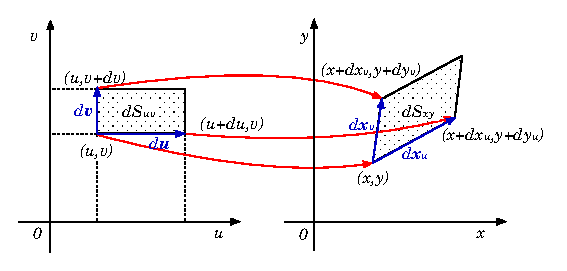
\includegraphics{Suv2Sxy.eps} }
    \caption{変数変換による矩形領域の変形}
    \label{fig:Suv2Sxy}
  \end{center}
\end{figure}
$\vect{u}$が$(u,v)$から$d\vect{u}=(du,0)$だけ変位したときの$\vect{x}$の
変位を$d\vect{x}_u$,
$(u,v)$から$d\vect{v}=(0,dv)$だけ変位したときの$\vect{x}$の変位を
$d\vect{x}_v$と書くと,次式が得られる。
\begin{align}
  d\vect{x}_u=
  \begin{pmatrix}
  \displaystyle\frac{dx}{du}\\
  \displaystyle\frac{dy}{du}
  \end{pmatrix}
  du,\quad
  d\vect{x}_v=
  \begin{pmatrix}
  \displaystyle\frac{dx}{dv}\\
  \displaystyle\frac{dy}{dv}
  \end{pmatrix}
  dv
\end{align}
よって,$uv$座標系において$(u,v)$を頂点として各軸に平行に2辺$d\vect{u}$および
$d\vect{v}$をとった長方形は, 
$xy$座標座標系上で$(x(u,v),y(u,v))$を頂点とし,
$d\vect{x}_u$と$d\vect{x}_v$を2辺とする平行四辺形に射影される(図\ref{fig:Suv2Sxy})
\footnote{変換$\vect{x}=\vect{x(\vect{u})}$の線形近似の範囲での話であ
  る。念のため。}。
$uv$平面上の微小長方形の面積$S_{uv}$は$dS_{uv}=dudv$で与えられるが
\footnote{正確に言うとこれはむしろ定義である。
  すなわちここでは,各座標系における\textbf{面積(体積)}を,
  各軸は直交するよう表し,各軸平行な辺をもつ長方形(直方体)は各辺の長さ
  を表す座標変位の積で表す。
  この場合$xy$座標系と$r\theta$座標系での面積は単位が異なることに注意
  せよ。},
これが$xy$平面に投影された微小平行四辺形の面積$dS_{xy}$は,
ベクトル積\footnote{
ここでは,各ベクトルに大きさ0の$z$軸成分を加えてベクトル積を計算する}
で求めることが出来る。
\begin{align}
dS_{xy}&=|d\vect{x}_u\times d\vect{x}_v|\notag\\
&=\left|\frac{\partial(x,y)}{\partial(u,v)}\right|dudv\notag\\
&=\left|\frac{\partial(x,y)}{\partial(u,v)}\right|dS_{uv}\notag
\end{align}
ここで,ヤコビアン行列の行列式
$\left|\frac{\partial(x,y)}{\partial(u,v)}\right|$を\bfindex{ヤコビアン}
(\nmindex{Jacobian})と呼ぶ。
上式より,座標変換によってある区間の面積は縮小拡大し,その拡大率がヤコ
ビアンで与えられることがわかる。

以上より以下のような積分公式を得られる。
\begin{align}
  \int_{S_{\vect{x}}}&f(x,y)dS_{xy}\notag\\
  &=\int_{S_{\vect{u}}}f(x(u,v),y(u,v))\left|\frac{\partial(x,y)}{\partial(u,v)}\right|dS_{uv}\notag
\end{align}
もしくは,
\begin{align}
  \int&\int_{S_{\vect{x}}}f(x,y)dxdy\notag\\
  &=\int\int_{S_{\vect{u}}}f(x(u,v),y(u,v))\left|\frac{\partial(x,y)}{\partial(u,v)}\right|dudv\notag
\end{align}
ただし,$xy$座標系での領域$S_{\vect{x}}$が$uv$座標系での領域
$S_{\vect{u}}$に対応しているとする。

さらに,3変数の場合についても同様に以下の積分公式が得られる。
ただし,2変数では面積と呼んでいた領域は,3変数では体積を表す。
\begin{align}
  \int_{V_{\vect{x}}}&f(\vect{x})dV_{xyz}\notag\\
  &=\int_{S_{\vect{u}}}f(\vect{x}(\vect{u}))
  \left|\frac{\partial(x,y,z)}{\partial(u,v,w)}\right|dV_{\vect{u}}\notag
\end{align}
もしくは,
\begin{align}
  \int\int\int_{V_{\vect{x}}}&f(\vect{x})dxdydz\notag\\
  &=\int\int\int_{V_{\vect{u}}}f(\vect{x}(\vect{u}))\left|\frac{\partial(x,y,z)}{\partial(u,v,w)}\right|dudvdz\notag
\end{align}

\question
\begin{enumerate}
\item 式(\ref{eq:circle-xy})にヤコビアンを用いた変数変換を行って
式(\ref{eq:circle-rtheta})を導きなさい。
\item $xyz$直交座標系による積分を3次元極座標系による積分に変換するには
  次式に従えばよいことを証明しなさい。
  \begin{align}
    \int&\int\int_{V_{\vect{x}}}f(x,y,z)dxdydz\notag\\
    &= \int\int\int_{V_{\vect{r}}}f(x,y,z)r^2\sin\theta\cos\phi dr d\theta d\phi\notag
  \end{align}
  ただし,極座標系での領域$V_{\vect{r}}$が直交座標系での領域
    $V_{\vect{x}}$に対応しているとする。
\item $xyz$直交座標系による積分を3次元円柱座標系による積分に変換する式
  を導きなさい。
\end{enumerate}% 

\subsection{ガウス分布の面積}
以下の積分を求めたい。
\begin{align}
  \label{eq:int_e}
  \int_{-\infty}^{\infty}e^{-x^2}dx
\end{align}

\begin{enumerate}
\item 上式が次式の平方根で与えられることを説明せよ。
  \begin{align}
    \label{eq:int_ee}
    \int_{-\infty}^{\infty}\int_{-\infty}^{\infty}e^{-(x^2+y^2)}dxdy
  \end{align}
\item 式(\ref{eq:int_ee})はどのような図形の体積を表しているか。図を書
  いて説明せよ。
\item 式(\ref{eq:int_ee})を$(x,y)$による積分から極座標$(r,\theta)$を用
  いた積分に変換せよ。
  その時,どのように考えて変換式を導いたかを図を用いて説明せよ。
\item 積分を実行して式(\ref{eq:int_e})の値を求めなさい。
\end{enumerate}% 

\section{最小二乗法}
\subsection{最小二乗法の解析的解法}

ある測定データ対$(x_i,y_i)$, $(i=1,...,n)$が得られたとき,
この測定データの真の分布が$y=c+dx$という線形関係にあると仮定して
$c,d$を推定する方法(\bfindex[たんかいきかいせき]{単回帰解析}, 
\nmindex{regression analysis})の一つ
に\bfindex[さいようにじょうほう]{最小二乗法}(
\nmindex{least mean square}, \nmindex{LMS})がある。
この方法は,真の分布$y=c+dx$に対する測定データのバラツキの2乗誤差
(次式)が最小になるように$c,d$を決める方法である。
\begin{align}
\label{eq:sqerr}
  E=\frac{1}{2}\sum_{i=1}^{n}(y_i-(c+dx_i))^2
\end{align}
\begin{enumerate}
\item 上式はデータのバラツキをどのような意味で最小にする式になっている
  か、その意味をグラフを描いて説明しなさい。
\item 式(\ref{eq:sqerr})を最小にする$c,d$を求めなさい。\\
ヒント)式(\ref{eq:sqerr})を$c,d$それぞれについて偏微分した値が0になる
ように$c,d$を決める。このとき,偏微分によって得られた式が
以下を満たすことに注目すると計算が簡単になる。
\begin{align}
  \label{eq:sol-minsq}
  \begin{pmatrix}
    \sum_i1   &  \sum_ix_i \\
    \sum_ix_i &  \sum_ix_i^2
  \end{pmatrix}
  \begin{pmatrix}
    c \\ d
  \end{pmatrix}
  =
  \begin{pmatrix}
    \sum_iy_i\\ \sum_ix_iy_i
  \end{pmatrix}
\end{align}
\end{enumerate}% 

\subsection{最小二乗法の幾何学的意味\prog}

\subsubsection{射影行列\prog}
\nquestion
ベクトル$\vect{b}$の$\vect{a}$への射影$\vect{p}$を以下のように求めなさ
い。
ただし,$\vect{a},\vect{b}\ne\vect{0}$とする。
\begin{enumerate}
\item $\vect{p}=k\vect{a}$, $\vect{e}=\vect{p}-\vect{b}$とおく。
  $\vect{e}$, $\vect{p}$, $\vect{b}$がどのような幾何学的関係になっている
  かを図示して説明しなさい。
\item $k$を求めなさい。
\item $\vect{p}$が以下のように表されることを示しなさい。
  \begin{align}
  \vect{p}&=P\vect{b}\notag\\
  P&=\frac{\vect{a}\vect{a}^T}{\vect{a}^T\vect{a}}\notag
  \end{align}
\end{enumerate}
\comment 上式で与えられる$P$を
\bfindex[しゃえいぎょうれつ]{射影行列}
(\nmindex{projection matrix})とよぶ。
$P$はベクトル空間内の点$\vect{b}$を$\vect{a}$上の点に射影する,言いか
えると$\vect{a}$上の点のうち$\vect{b}$からの距離がもっとも近い点に写像
する行列である。

\nquestion
$m\times n$行列$A$の列ベクトル$\vect{a}_1,\vect{a}_2, \cdots, \vect{a}_n$
が作るベクトル空間へのベクトル$\vect{b}$の$C(A)$への射影$\vect{p}$を以
下のように求めなさい。
\begin{enumerate}
\item $C(A)$内の任意の点は$A\vect{x}$で表現できることを説明しなさい。
\item $\vect{p}=A\vect{x}$, $\vect{e}=\vect{p}-\vect{b}$とおく。
  $\vect{e}$が$\vect{a}_1,\vect{a}_2, \cdots, \vect{a}_n$ と直交するこ
  とから,以下が成り立つことを説明しなさい。
  \begin{align}
    A^T(\vect{p}-\vect{b})=\vect{0}\notag
  \end{align}
\item 次式が成り立つことを示しなさい。
ただし,$A^TA$は逆行列をもつとする。
  \begin{align}
    \vect{p}&=P\vect{b}\notag\\
    \label{eq:projection}
    P&=A(A^TA)^{-1}A^T
  \end{align}
\item 
  $A$の列ベクトルが互いに一次独立な時,すなわち$A\vect{x}=\vect{0}$が
  $\vect{x}=\vect{0}$に対してのみ成立するとき,$A^TA$は逆行列をもつ。
  このことを証明せよ。\\
  ヒント)$A^TA$が正則ではない,すなわち
  \begin{align}
    \exists \vect{x}\ne 0,\quad  A^TA\vect{x}=0\notag
  \end{align}
と仮定すると,$A\vect{x}=0$となり$A$の列ベクトルが独
  立であるという前提に反することを証明すればよい。
\item 式(\ref{eq:projection})で与えられる射影行列$P$について以下を証明しなさい。
  幾何学的意味も説明しなさい。
  \begin{enumerate}
  \item $P^2=P$
  \item $\forall \vect{x}\in C(A), P\vect{x}=\vect{x}$
  \item $\forall \vect{x}\in N(A), P\vect{x}=\vect{0}$
  \end{enumerate}
\end{enumerate}
$P$はベクトル空間内の点$\vect{b}$を$C(A)$上に射影する、言い替えると
$C(A)$上の点のうち$\vect{b}$からの距離が最も近い点に写像する行列である。% 

\subsubsection{最小二乗法の幾何学的意味\label{sec:single-regression}\prog}

方程式
\begin{align}
  A\vect{x}=\vect{b}\notag
\end{align}
は,$\rank A\ne\rank[A|b]$のとき解を持たない。
このとき$\vect{b}$を$C(A)$に射影したベクトルを$\hat{\vect{b}}$とすると,
\begin{align}
  A\hat{\vect{x}}=\hat{\vect{b}}\notag
\end{align}
を満たす近似解$\hat{\vect{x}}$を得ることができる。
近似解は
式(\ref{eq:projection})で与えられる射影行列$P$を用いると次式の解になる。
\begin{align}
  \label{eq:sol2-minsq}
  A^TA\hat{\vect{x}}=A^T\hat{\vect{b}},\quad \hat{\vect{b}}=P\vect{b}
\end{align}
\question
観測データ対$(x_i,y_i)$, $(i=1,...,n)$が真の分布$y=c+dx$に従うとする
と,観測ノイズがなければ次式より$c,d$を求めることができる。
\begin{align}
  A\vect{x}=\vect{b}\notag
% +\vect{e}\notag\\
%   &=\hat{\vect{b}}\notag
\end{align}
\begin{align}
  A&=\begin{pmatrix}
    1 & x_1\\
    1 & x_2\\
    \vdots & \vdots \\
    1 & x_n
  \end{pmatrix},\quad
  \vect{x}=
  \begin{pmatrix}
    c \\ d
  \end{pmatrix},\quad
  \vect{b}=
  \begin{pmatrix}
    y_1 \\ y_2 \\\vdots \\ y_n
  \end{pmatrix}\notag
\end{align}
しかし、実験データを処理するときには多くの場合
$\rank A\ne\rank[A|b]$となり解$(c,d)$を得ることができない。
このとき
上式の$\vect{b}$を$C(A)$に射影した$\hat{\vect{b}}$が真の値とみなせば,
言いかえると点$\hat{\vect{b}}$に対する真の点は
$C(A)$内で最も$\hat{\vect{b}}$から近い点とみなせば,
解を得ることができる。
その解が式(\ref{eq:sol-minsq})で得られるものと等しいである
ことを証明しなさい。\\
ヒント) 式(\ref{eq:sol-minsq})と式(\ref{eq:sol2-minsq})が等価であることを示せ
ば良い。

% \subsubsection{最小二乗法の別解$^*$}

% 測定データ対$(x_i,y_i)$, $(i=1,...,n)$が
% 真の分布$y=c+dx$に従うとき,$e_i=(c+dx_i)-y_i$とおくと次式を得る。
% \begin{align}
%   &\vect{e}=A\vect{x}-\vect{b}\notag\\
%   A&=\begin{pmatrix}
%     1 & x_1\\
%     1 & x_2\\
%     \vdots & \vdots \\
%     1 & x_n
%   \end{pmatrix}
% \end{align}
% 最小二乗法とは$\vect{e}^T=(A\vect{x}-\vect{b})^T(A\vect{x}-\vect{b})$
% を最小にする解
% の近似解のうち,式(\ref{eq:sqerr})を最小にするものを求める方法である。% 

\subsubsection{重回帰分析\label{sec:multi-regression}\prog}
観測データ$(x_{1i},x_{2i},y_i)$, $(i=1,...,n)$が分布$y=c+dx_1+ex_2$に従うとする。
このとき$c,d,e$も前問と同様に求めることができる。すなわち,
\begin{align}
  &A\vect{x}=\vect{b}\notag\\
  A&=\begin{pmatrix}
    1 & x_{11} & x_{21}\\
    1 & x_{12} & x_{22}\\
    \vdots & \vdots & \vdots \\
    1 & x_{1n} & x_{2n}
  \end{pmatrix},\quad
  \vect{x}=
  \begin{pmatrix}
    c \\ d \\e
  \end{pmatrix},\quad
  \vect{b}=
  \begin{pmatrix}
    y_1 \\ y_2 \\\vdots \\ y_n
  \end{pmatrix}\notag
\end{align}
に対して,式(\ref{eq:sol2-minsq})を満たす解を求めれば良い。
このように複数の観測変数の間に線形関係があると仮定して、
その係数を求める方法を\bfindex[じゅうかいきぶんせき]{重回帰分析}という。

\question
式(\ref{eq:sol2-minsq})は多変数の観測データ$(x_{1i},x_{2i},y_i)$,
$(i=1,...,n)$に対して以下のように書けることを示しなさい。
\begin{align}
  \label{eq:multi-regression}
  A^TA\hat{\vect{x}}&=A^T\hat{\vect{b}}\\
  A^TA&=
  \begin{pmatrix}
    \sum_i1   &  \sum_ix_{1i} &  \sum_ix_{2i} \\
    \sum_ix_{1i} &  \sum_ix_{1i}^2 &  \sum_ix_{1i}x_{2i} \\
    \sum_ix_{2i} &  \sum_ix_{1i}x_{2i} & \sum_ix_{2i}^2 
  \end{pmatrix}\notag\\
  A^T\hat{\vect{b}}
  &=A^TP\vect{b}=
  \begin{pmatrix}
    \sum_iy_i\\ \sum_ix_{1i}y_i\\ \sum_ix_{2i}y_i
  \end{pmatrix}\notag
\end{align}
\comment
上式で,$A^TA$を
\bfindex[ぶんさんきょうぶんさんぎょうれつ]{分散・共分散行列}
(\nmindex{variance-covariance matrix})とよぶ。
ベクトル$\vect{x}_1,\vect{x}_2$の直交性が低いとき(データの相関が高い
とき)には$\det(A^TA)$は0に近くなる。
この場合には$\vect{x}$はノイズに敏感に反応する信頼性の低い値になってしまう。% 

\subsection{擬似逆行列\prog}
$m\times n$, ($m>n$)行列$A$が与えられたとき$A$は逆行列を持たない。
しかし,\ref{sec:single-regression},\ref{sec:multi-regression}節でふ
れたように$A$が一次独立な列ベクトルをもつならば$A^TA$は常に逆行列をもつ。
そこで$A\vect{x}=\vect{b}$が解を持つとき,その解は以下のように求めるこ
とが出来る。
\begin{align}
  A^TA{\vect{x}}&=A^T{\vect{b}}\notag\\
  {\vect{x}}&=(A^TA)^{-1}A^T{\vect{b}}\notag
\end{align}
ここで, $A^{+}=(A^TA)^{-1}A^T$を$A$の
\textbf{左擬似逆行列}\index{ぎじぎゃくぎょうれつ@疑似逆行列!ひだり@左---}
\index{ぎじぎゃくぎょうれつ@疑似逆行列}
(\nmindex{pseudo-inverse matrix})とよぶ。 

\question
\begin{enumerate}
\item $A^{+}A=I$を証明しなさい。
\item $AA^{+}A=A$を証明しなさい。
\item $AA^{+}$が$C(A)$への射影行列であることを示しなさい。
  このことから$AA^{+}A=A$の意味を幾何学的意味を説明しなさい。
\end{enumerate}

\comment
$m\times n$行列$A$の列ベクトルが一次従属であれば 
$A^TA$は逆行列をもたない。
しかし、この場合にも$A^+A=I$, ($I=\diag\{1,\cdots,1,0,\cdots,0\}$は
$r=\rank A$
個の非零成分をもつ)をみたす擬似逆行列$A^+$を定義できる。
詳細は主成分分析に関する文献を参照すること。

%%%%%%%%%%%%%%%%%%%%%%%%%%%%%%%%%%%%%%%%%%%%%%%%%%%%%%%%%%%%%%%%%% 
\section{統計}

\subsection{平均,分散}
ある測定データ$x_i$, $(i=1,...,n)$がガウス分布に従っているとする。
データの平均値および二乗平均値を
\begin{align}
<x>=\frac{1}{n}\sum_{i=1}^nx_i,\quad
<x^2>=\frac{1}{n}\sum_{i=1}^nx_i^2\notag
\end{align}
と定義する。
データと平均値の差の自乗平均を,\bfindex[ぶんさん]{分散}$\sigma^2$とよ
ぶ。
すなわち,
\begin{align}
\sigma^2=\frac{1}{n}\sum_{i=1}^n(x_i-<x>)^2.\notag
\end{align}
このとき,次式が成り立つことを証明せよ。
\begin{align}
\sigma^2=\frac{1}{n}\sum_{i=1}^n(x_i-<x>)^2=<x^2>-<x>^2.\notag
\end{align}
\textbf{コメント:}上式で定義される分散を
\bfindex[ひょうほんぶんさん]{標本分散}という。 
分散を求めるときに大きな問題になるのは,真の平均値
(\bfindex[ぼへいきん]{母平均})を
知らないまま計算しないといけないことである。
上式では,平均値$<x>$と$n$個のデータ$x_i$の合計$n+1$個の変数が
存在するが,平均値$<x>$は$x_i$から決まるので,実はデータの自由度は$n$
である。そこで,平均値$<x>$と$n-1$個のデータから分散は求められると考え
て定義されたのが次式の\bfindex[ふへんぶんさん]{不偏分散}であり,
標本分散よりもより良い,真の分散(\bfindex[ぼぶんさん]{母分散})の推定値を
得ることができる。
\begin{align}
\sigma^2=\frac{1}{n-1}\sum_{i=1}^n(x_i-<x>)^2\notag
\end{align}
% 

\subsection{ガウス分布の確率密度関数}
ガウス分布の確率密度関数は次式で与えられる。
\begin{align}
  \label{eq:prob}
  P(x)=Ae^{-\frac{x^2}{2\sigma^2}}
\end{align}
ここで,「$P(x)$が\bfindex[かくりつみつどかんすう]{確率密度関数}である」とは,
$x\sim x+dx$のデータ発生確率が
$P(x)dx$で与えられることを意味する。
\begin{enumerate}
\item $x\in (-\infty,\infty)$のデータ発生確率は1であるので,
  次式が成立する。
  \begin{align}
    \int_{-\infty}^{\infty} P(x)dx=1\notag
  \end{align}
  このことから式(\ref{eq:prob})の$A$の値を求めよ。
\item この確率密度関数にしたがって得られるデータの期待値が$0$である
  ことを示しなさい。
\item この確率密度関数にしたがって得られるデータの分散を求めなさい。
\item \bfindex[ひょうじゅんへんさ]{標準偏差}$\sigma$は
  \textbf{分散}$\sigma^2$の平方根で与
  えられる。 ある測定データがガウス分布にしたがうとき,
  平均値のまわり$\sigma$, $2\sigma$, $3\sigma$の範囲に入るデータ数は
  データ全体のどの程度の割合を占めるかを計算したい。
  計算式を導け。実際に数値計算により答を求め,図示して説明せよ。
\end{enumerate}

%% \nquestion
%% リンゴに含まれる窒素の量を測定して次のようなデータを得た。この平均
%% 値と標準偏差$s$を計算せよ。次に平均値の周り$s$,$2s$,$3s$の範囲に入
%% るデータ数を数え,全体に対する割合をそれぞれ求めよ。
%% {\small
%% \begin{verbatim}
%% 2.10    2.82    2.17    1.99    2.22    3.09
%% 2.47    2.52    2.80    2.10    2.92    2.20
%% 1.75    2.77    2.82    2.67    3.05    2.93
%% 2.94    1.98    2.38    2.65    2.77    1.85
%% 1.69    2.70    2.68    2.06    2.36    2.28
%% 2.75    2.43    2.39    2.55    1.80    1.96
%% \end{verbatim}}% 

\section{確率}
\begin{enumerate}
\item 
  $[0,1]$の一様乱数を一度発生したとき,その値の2乗が$1/2$以下になる確
  率を求めよ。
\item 
  $[0,1]$の一様乱数を二度発生したとき,その値の2乗和が$1$以下になる確
  率を求めよ。
\item 間隔$d$で平行線がたくさん描かれている紙に,長さ$l$の針に落とした。
  この針が平行線と交わる確率を求めよ
  (\bfindex[びゅふぉんのはり]{ビュフォンの針})。
\end{enumerate}

\onecolumn
\pagestyle{plain}% 

\appendix
\section{TODO}
西井用のメモコーナーです。見ないで下さい\verb|(^^);;|
\begin{enumerate}
\item 確率から情報量につなげる問題
\end{enumerate}% 


\section{このドキュメントの著作権について}

\begin{enumerate}
\item 本稿の著作権は西井淳\url{nishii@sci.yamaguchi-u.ac.jp}が有します。
\item 非商用目的での複製は許可しますが,修正を加えた場合は必ず修正点および加筆者の
氏名・連絡先,修正した日付を明記してください。また本著作権表示の削除は行っ
てはいけません。
\item 本稿に含まれている間違い等によりなんらかの被害を被ったとしても著者は一切
責任を負いません。
\end{enumerate}
間違い等の連絡や加筆修正要望等の連絡は大歓迎です。

%% \newpage
%% \section{在庫中の問題}
%% \subsection{全微分}

%% おもりを糸で吊したとき,おもりが重力で揺れる周期$T$は,
%% その糸の長さを$l$とすると
%% \begin{align}
%%   T=2\pi\sqrt{\frac{l}{g}}\notag
%% \end{align}
%% で表される。ここで$g$は重力の大きさを表す定数(重力加速度の大きさ)である。
%% 糸の長さ$l$と重力加速度の大きさ$g$がそれぞれ微小量$dl$,
%% $dg$変化した時の周期$T$の変化の割合$dT/T$を求めよ。($T$の全微分を求めればよい)。

\printindex% 

\end{document}
